%opening
The high energy photons radiated from electrons in the target can decay into electron-positron pairs. These electrons can also be detected by the spectrometers and we cannot distinguish them from the scattering electrons just base on their performance in the detectors. To determine the magnitude of this background and eliminate them from our data, we can use the charge-symmetric features of this background and just measure the positrons yields to meet our goals with the following relations
\begin{equation}\label{postiron_eq1}
\dfrac{Y_{e-}^{BK}}{Y_{e-}^{tot}}=\dfrac{Y_{e-}^{BK}}{Y_{e-}^{BK}+Y_{e-}^{DIS}}=\dfrac{Y_{e+}^{BK}}{Y_{e+}^{BK}+Y_{e-}^{DIS}}
\end{equation}  
Where the $Y_{e-}^{DIS}$ is the electron yield from deep inelastic scattering and $Y_{e+}^{BK}$ /$Y_{e-}^{DIS}$ is the positron(electron) yield from background

For MARATHON, positron measurements is performed at KIN1, KIN3, KIN5 for H3 , D2,He3 as well as empty cell and KIN1 ,KIN3 for H1. And Yields for the positron data is 
\begin{equation}\label{postiron_eq2}
Y_{e+}^{BK}=\dfrac{N_{e+}}{C*LT*\rho} \times Correction
\end{equation} 
Where $N_{e+}$ is the number of prositron, $LT$ is dead time correction ,C is the charge and $\rho$ is the density of the target.for positron analysis, the correcrtion include the endcap contimanation and non-positron contimation correction. Enpcap contimanation is similar with the electron analysis(See SectionXXX). To eliminate the non-positron background contimation, a combined exponential function for the background and a gauss peak function for the postion signal are used to fit the calorimeter E/P spectrum, the integration of the background tail beyond the E/P cut can be tread as the non-positron background(Fig \ref{po_1}).
\begin{figure}
 	\begin{center}
 		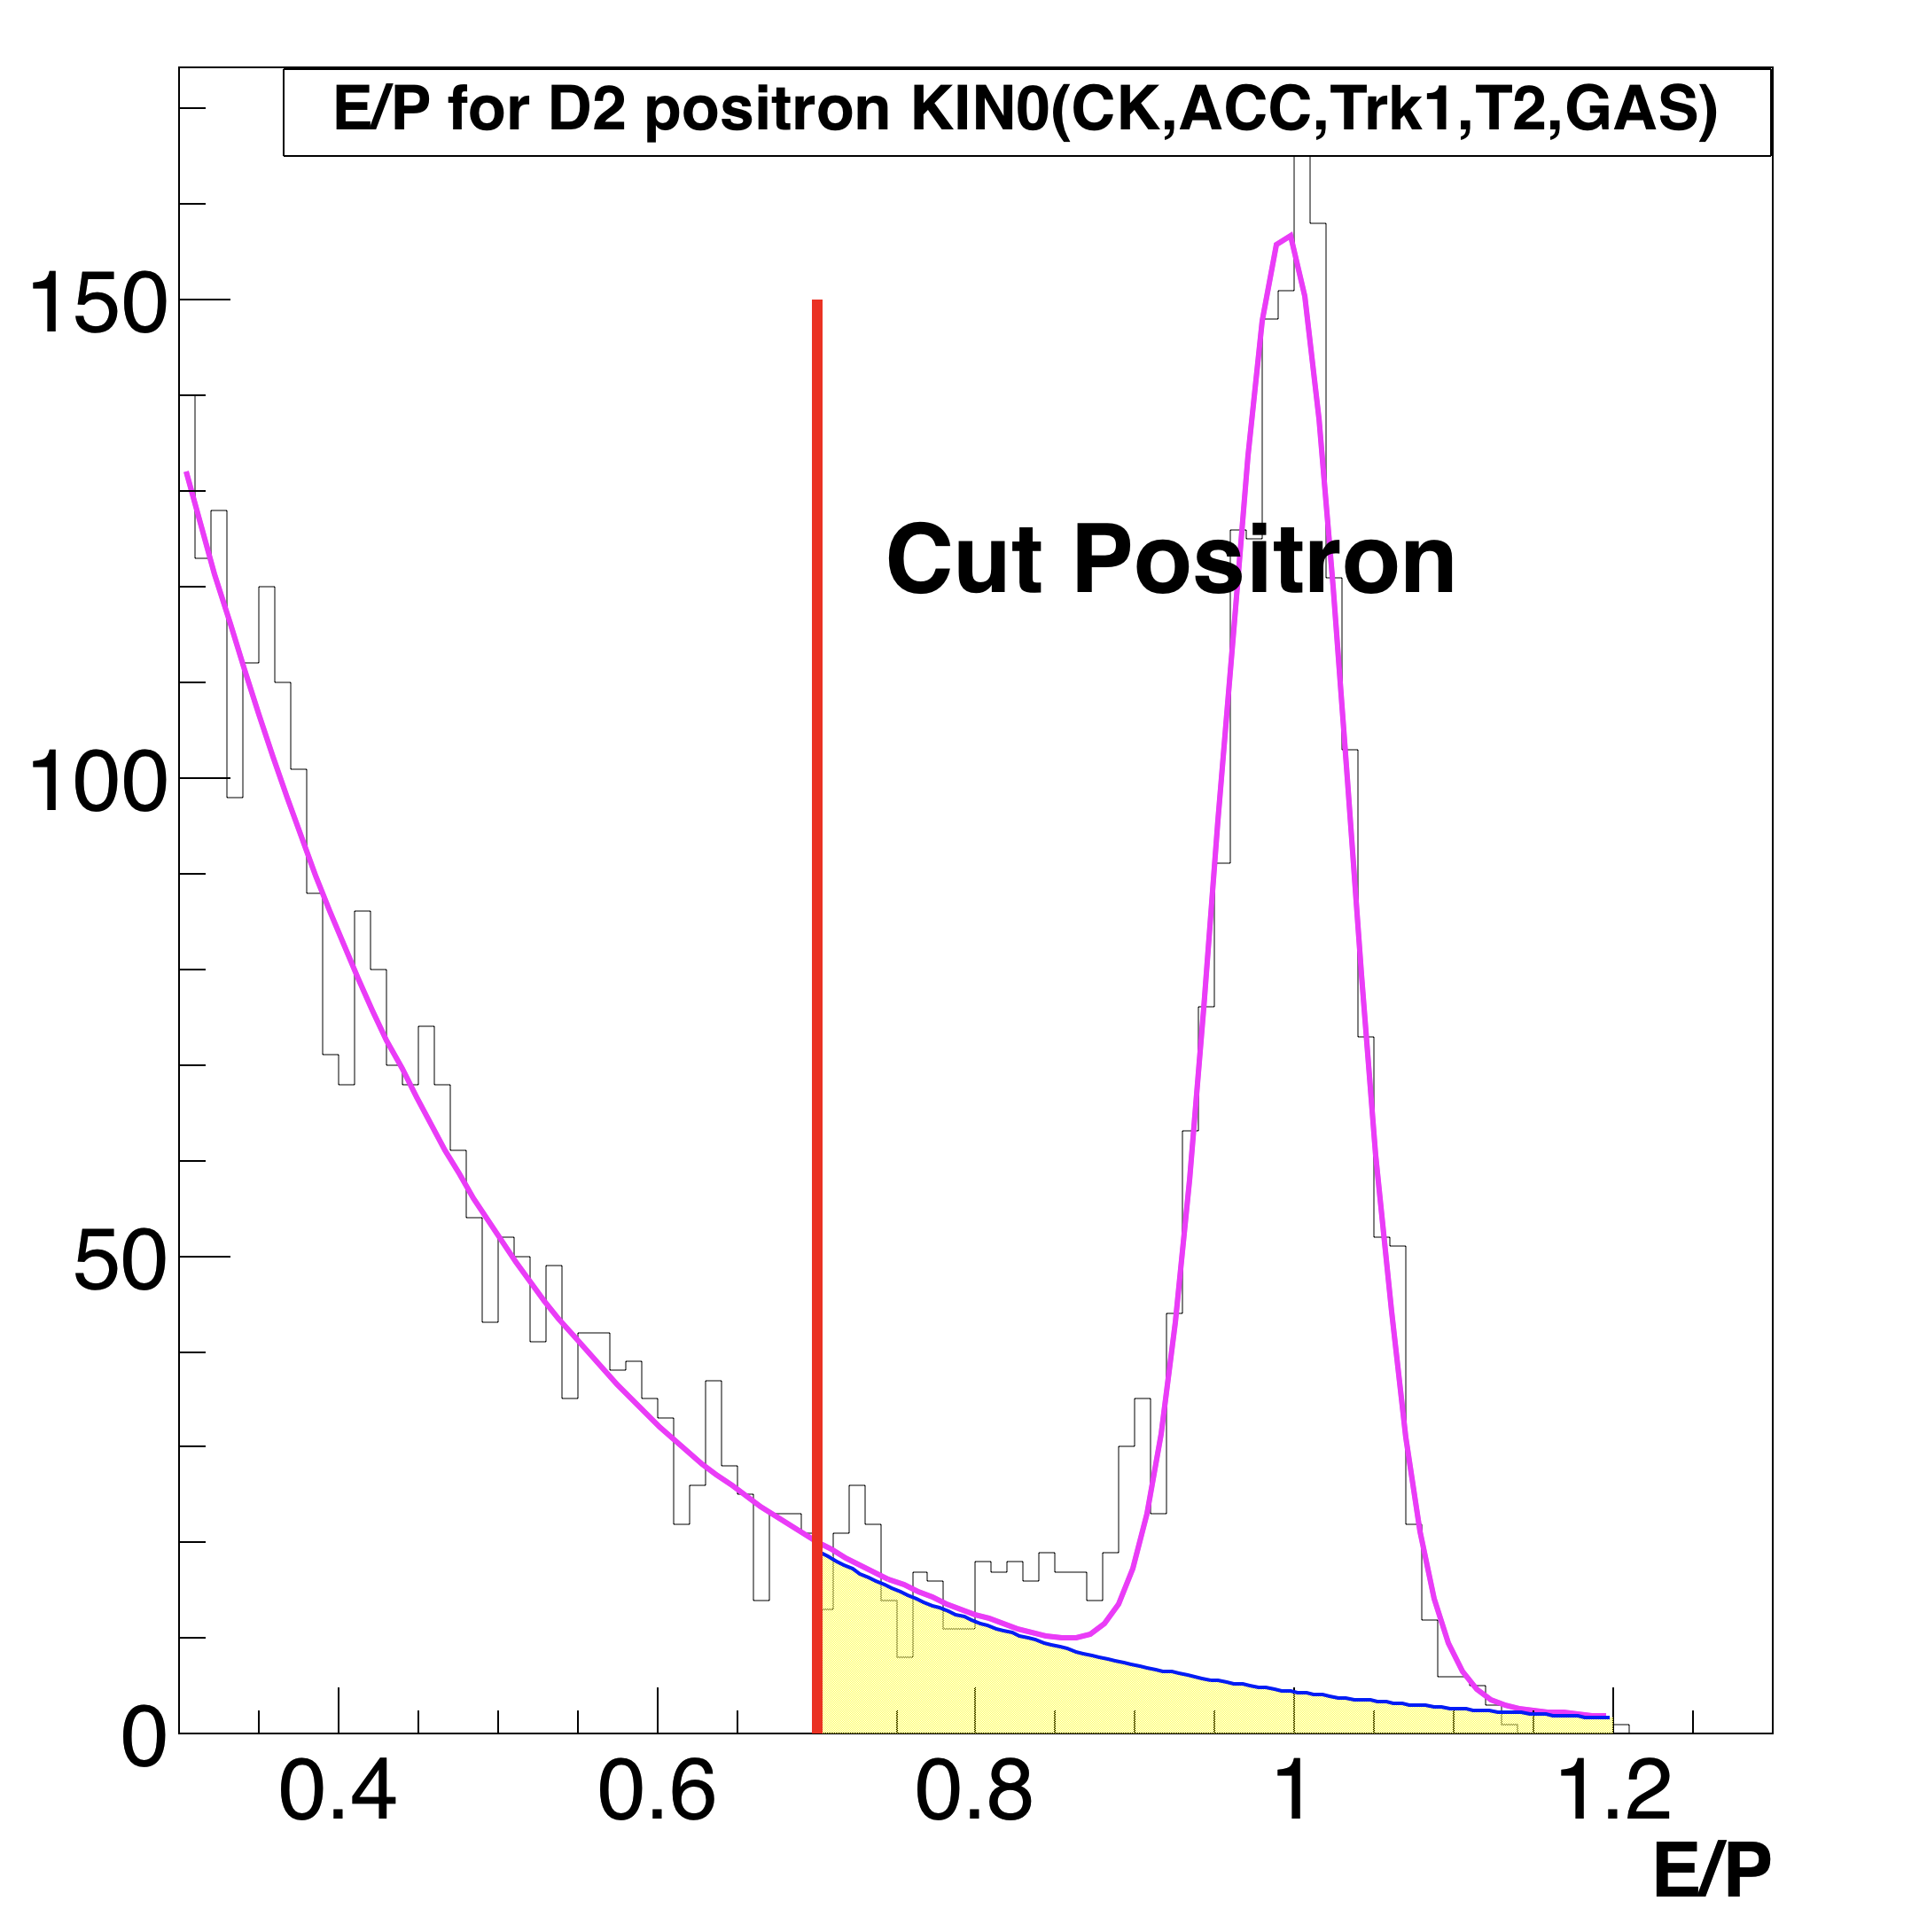
\includegraphics[width=0.4\textwidth] {./Positron_plot/Positron_1.png}
 		\caption{ The E/P spectrum for the KIN1 positron data , and the integration area of the expoential function( yellow shadow part) is the non-positron cotimatination} \label{po_1}
 	\end{center}
\end{figure}   

Combine with electrons with the corresponding kinematics settings, we can get the $Y_{e+}^{BK}/Y_{e-}^{tot}$, then a exponential function $f(x)=Ae_{-Bx}$ is performed to fit the $Y_{e+}^{BK}/Y_{e-}^{tot}$ . With this fitting function, charged-symmetric background be get rid of by 
\begin{equation}\label{postiron_eq1}
Y_{e-}^{DIS}=Y_{e-}^{tot}*\left(1-\dfrac{Y_{e+}^{BK}}{Y_{e-}^{tot}}\right)
\end{equation}  
\begin{figure}
 	\begin{center}
 		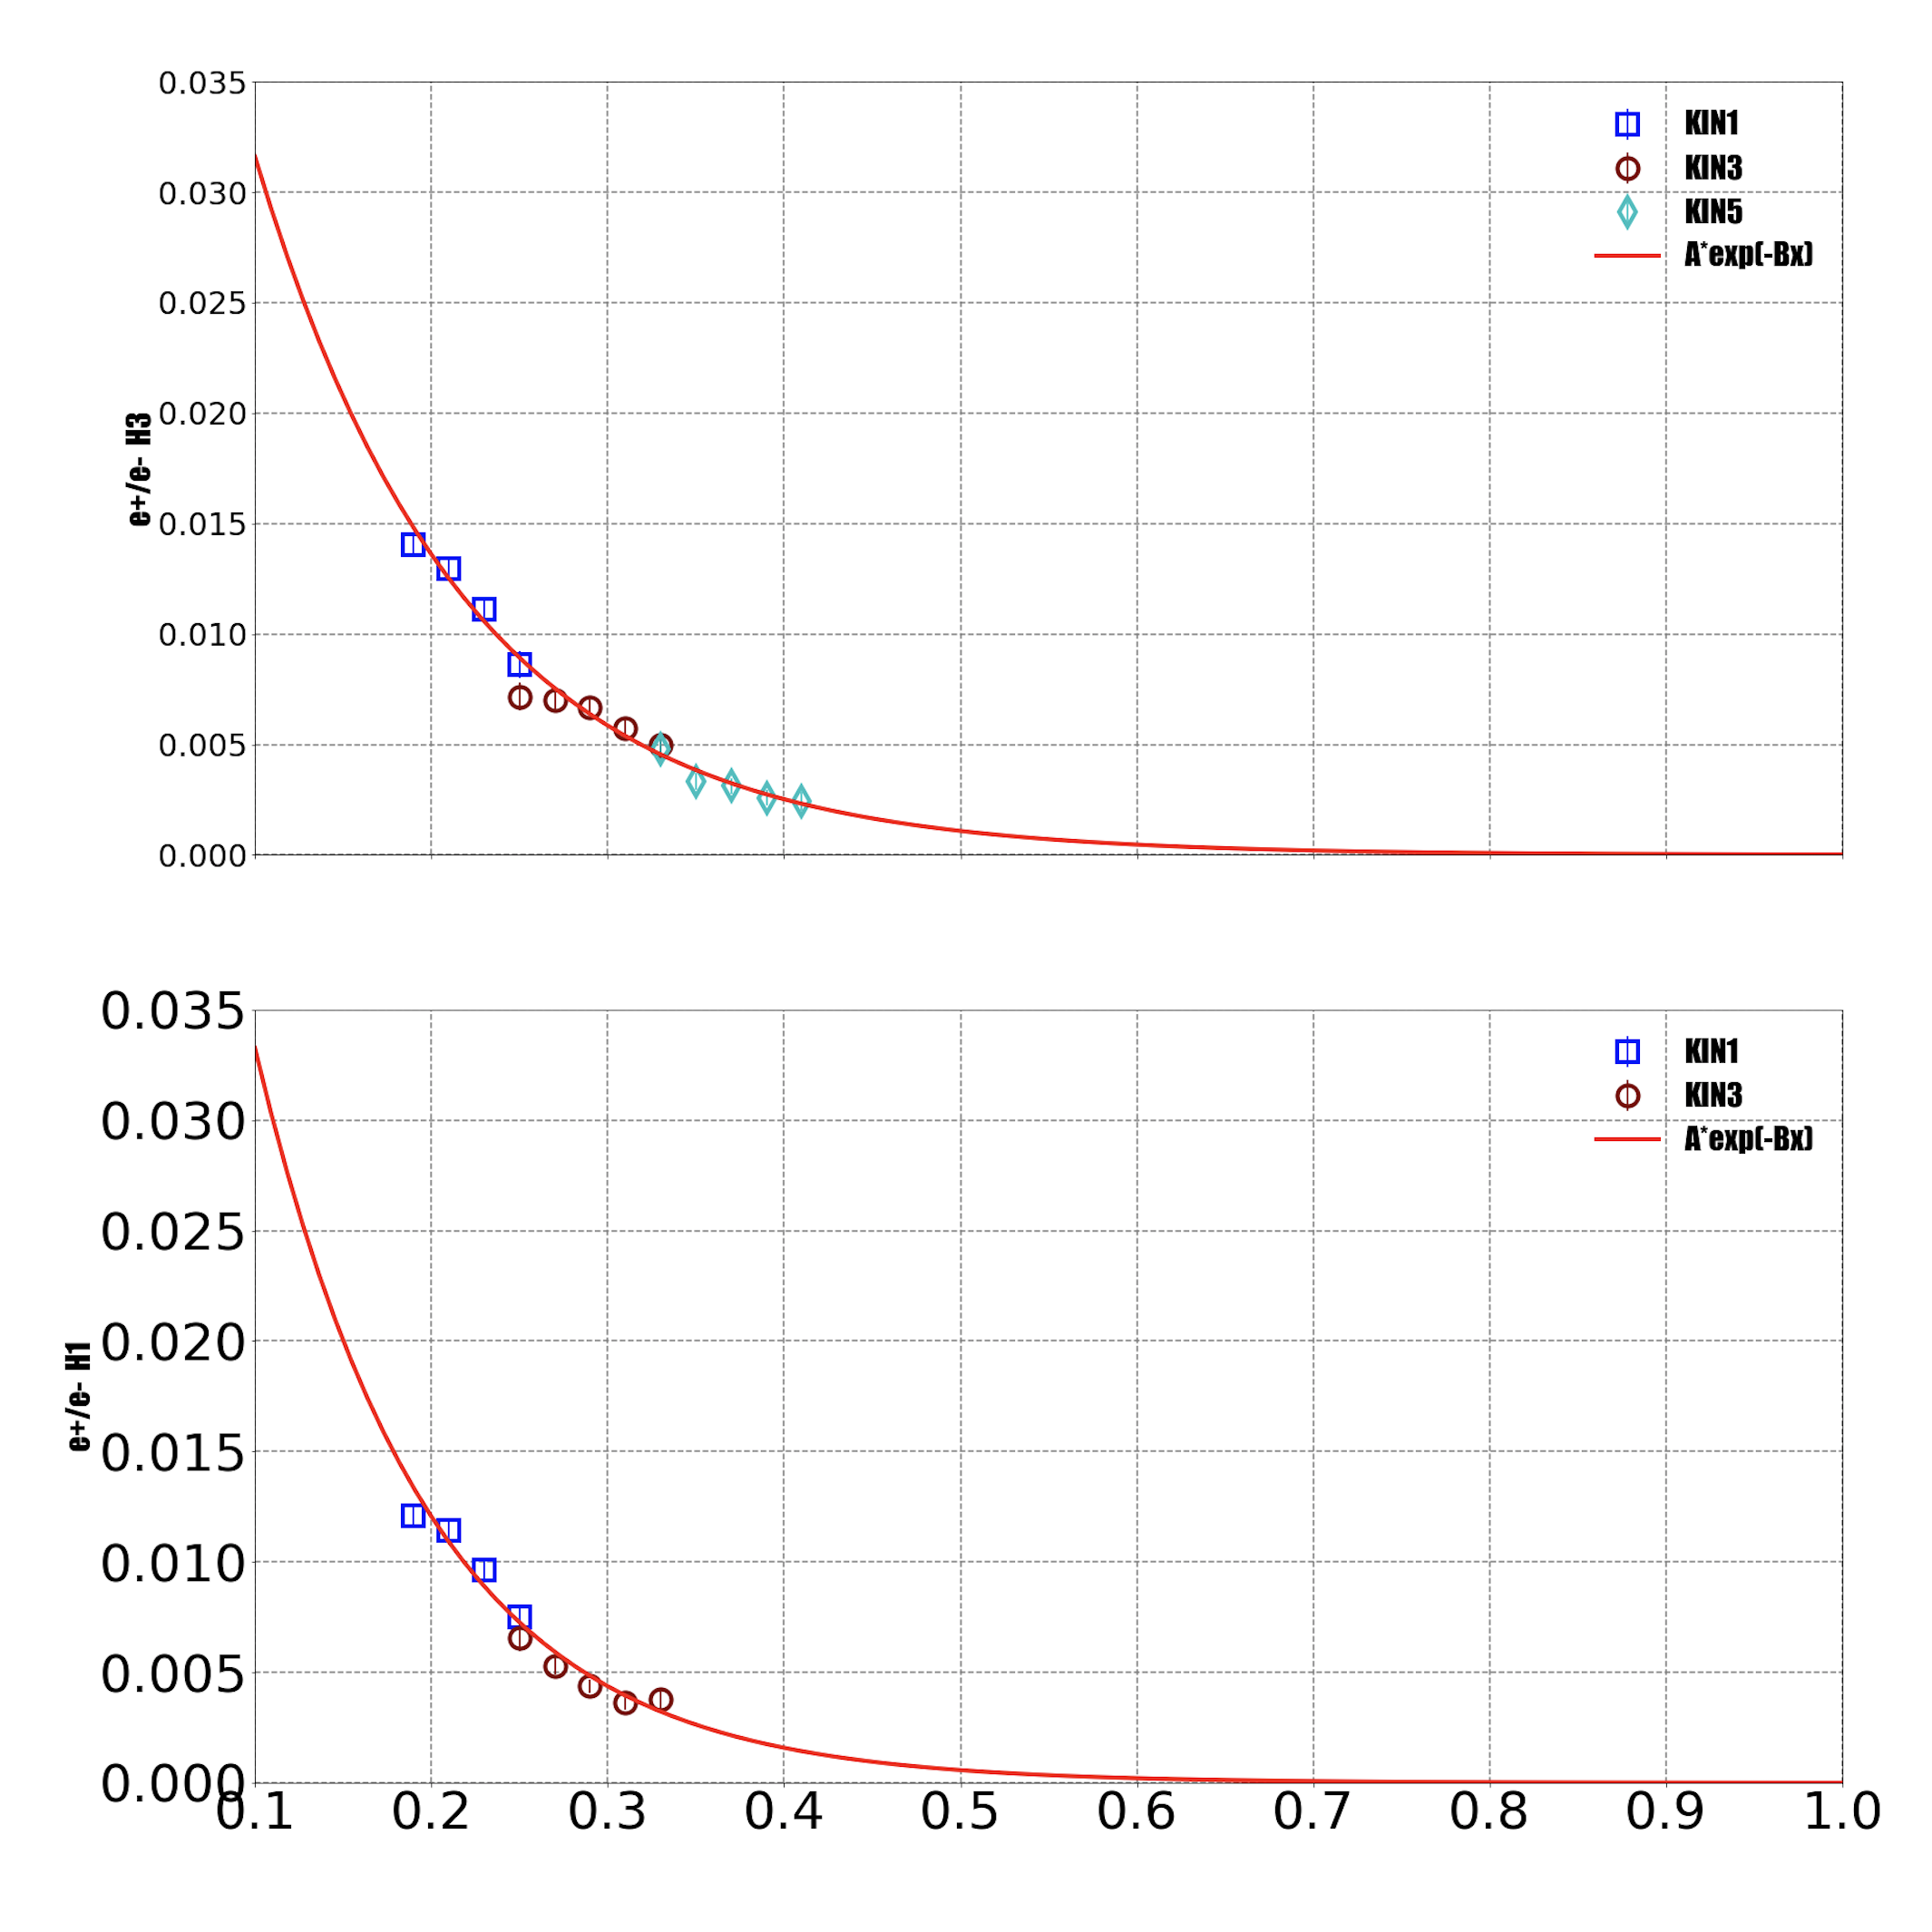
\includegraphics[width=0.4\textwidth] {./Positron_plot/Positron_2.png}
 		\caption{ Fig note : e+/e- for all the $^{1}H$ and $^{3}H$  target .An exponential fitting function is to performed to the data and fitting function is extended to the full Bejuken-x range for MARATHON data. } \label{po_2}
 	\end{center}
\end{figure}   
  
\begin{figure}
 	\begin{center}
 		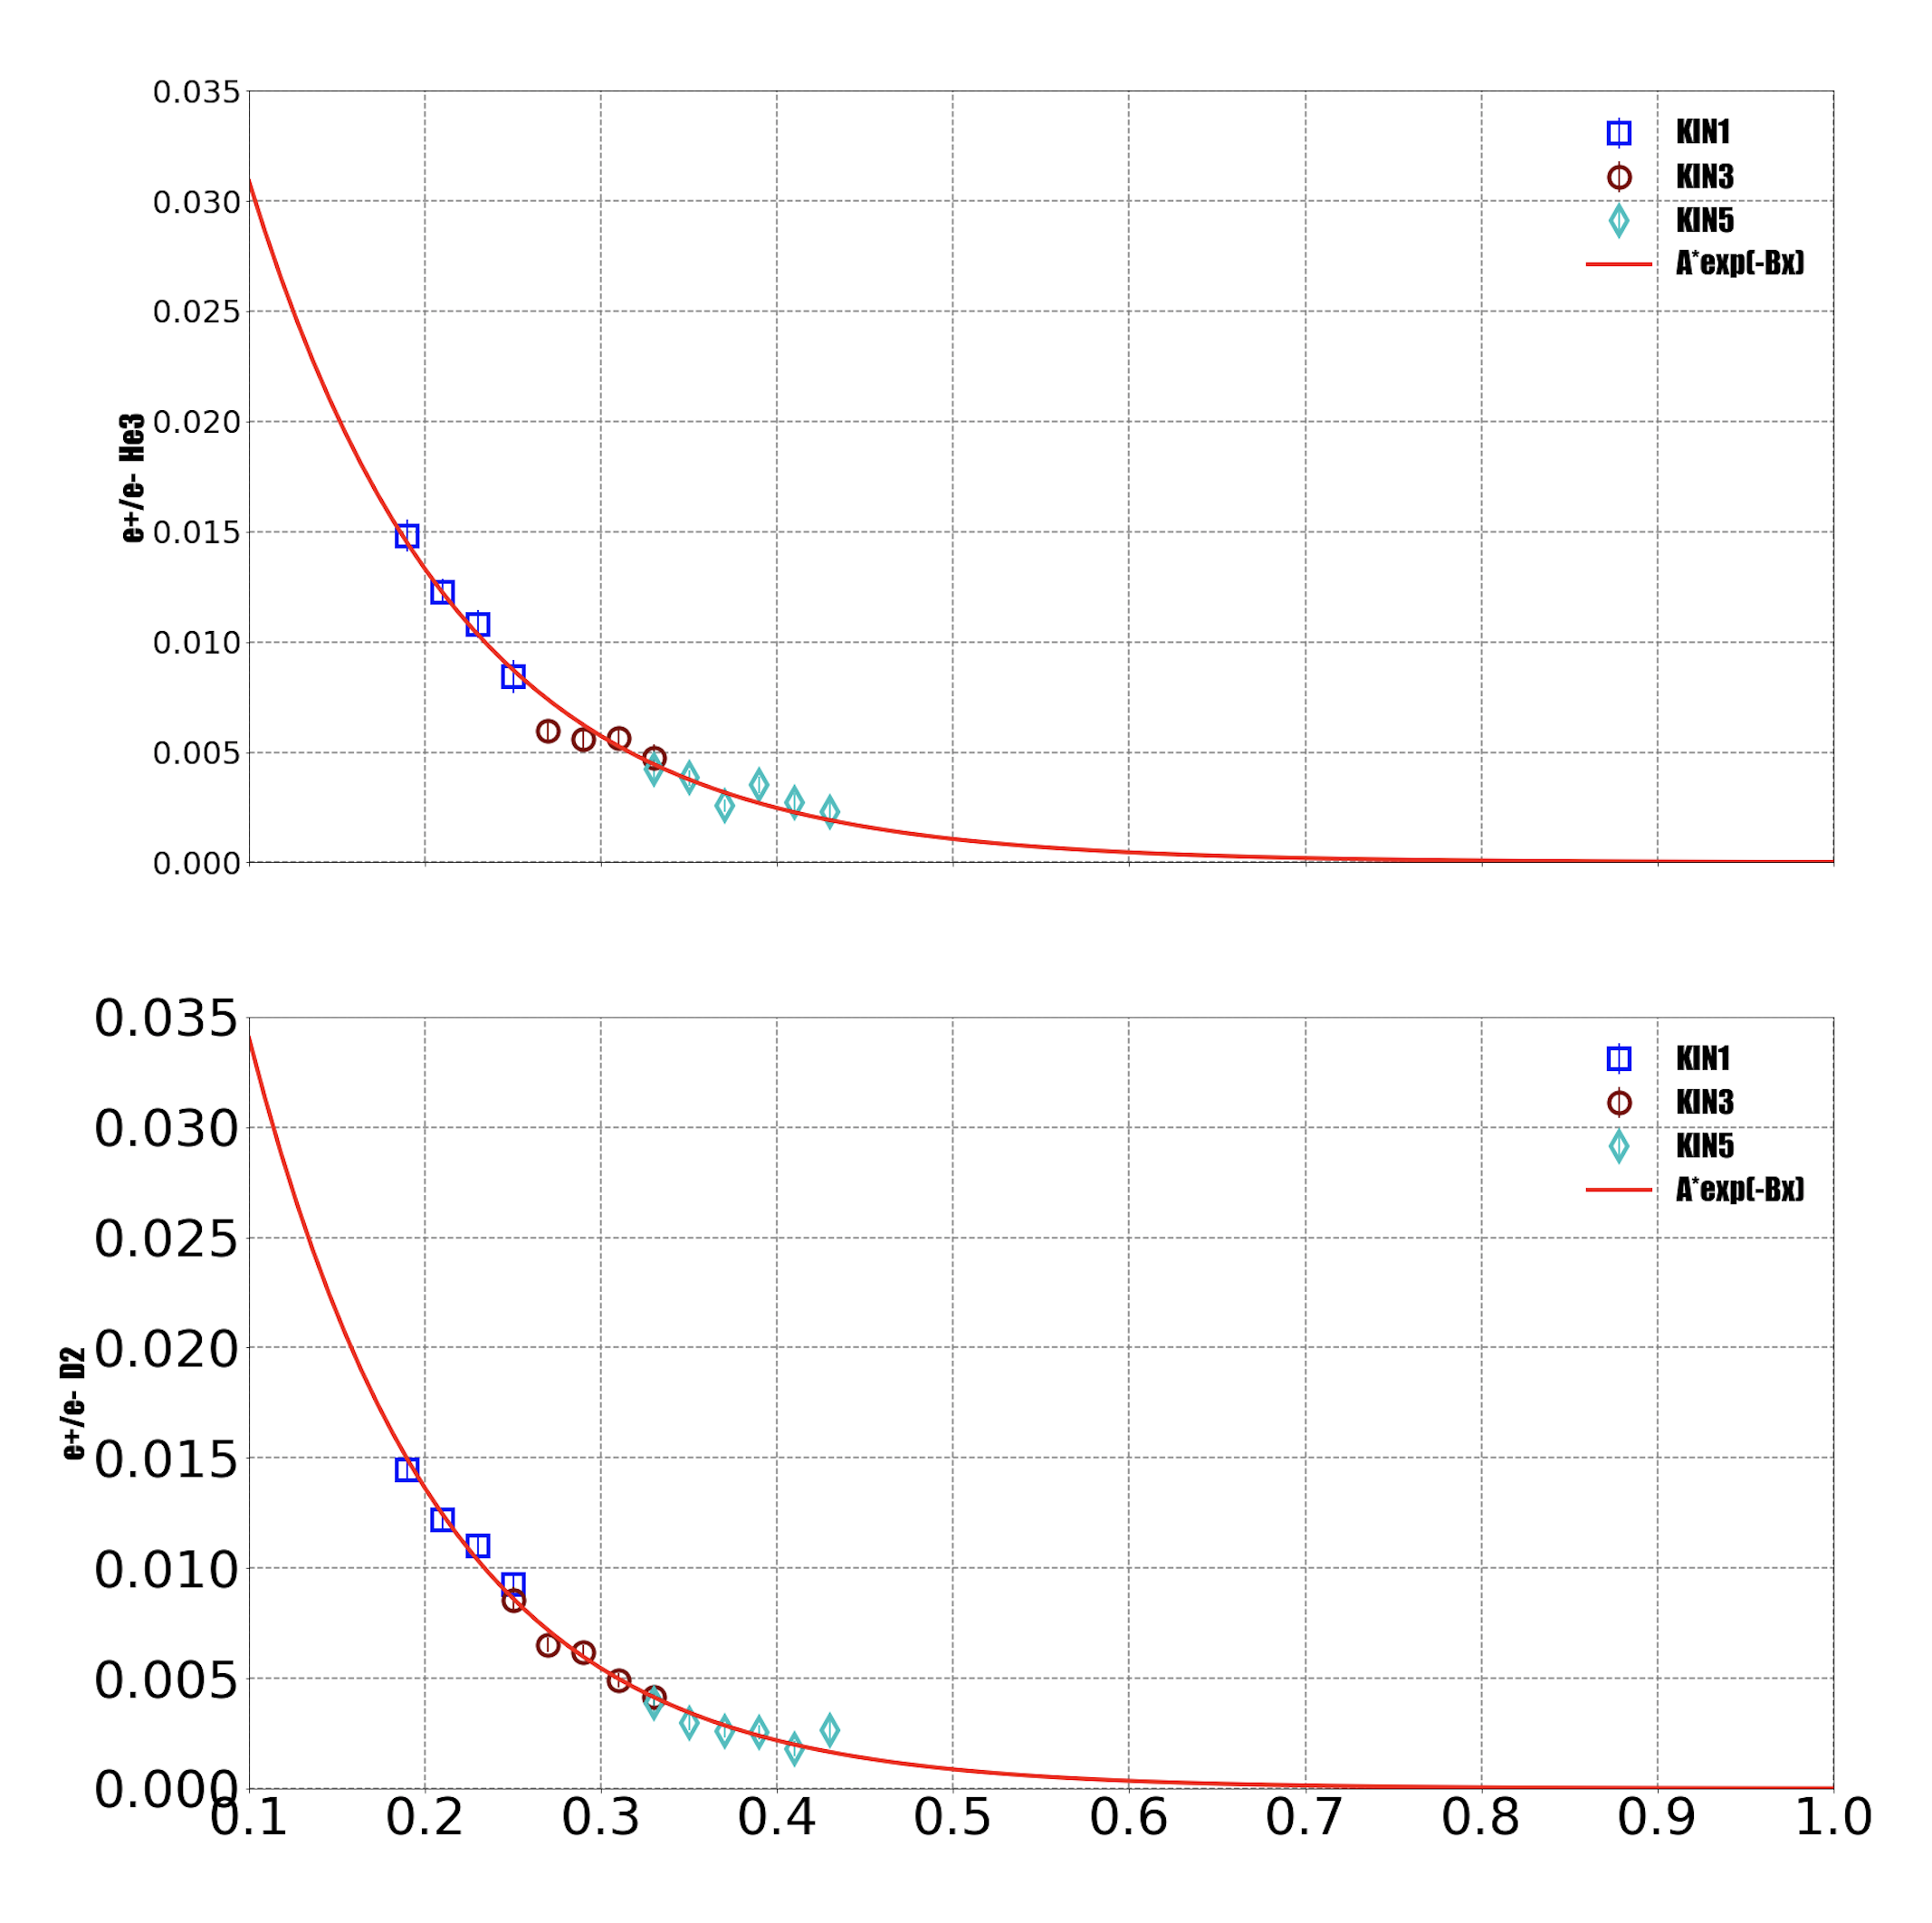
\includegraphics[width=0.4\textwidth] {./Positron_plot/Positron_3.png}
 		\caption{ Fig note : e+/e- for all the $^{3}He$ and $^{2}D$  target .An exponential fitting function is to performed to the data and fitting function is extended to the full Bejuken-x range for MARATHON data. } \label{po_3}
 	\end{center}
\end{figure}  

